% Time-stamp: <2025-05-15 01:26:31 okumura>
\documentclass{jarticle}

\usepackage{tam}
\usepackage{fleqn}
\usepackage{url}
\usepackage{bm}
\usepackage[dvipdfmx]{graphicx}
\usepackage[dvipdfmx]{color}
%\usepackage{color}
\usepackage{colordef}
\usepackage{amssymb}
\usepackage{pdfpages}
\usepackage{ulem}

%%%%%%%%%% Command alias %%%%%%%%%%
\newcommand{\IB}{$\bullet$}
\newcommand{\IC}{$\circ$}
\newcommand{\IS}{$*$}
%%%%%%%%%%%%%%%%%%%%%%%%%%%%%%%%%%%

\title{買電と自己託送を考慮した電力運用最適化モデル}
\author{神戸大学大学院 奥村侑真}
\date{}

\def\baselinestretch{1.02}
\renewcommand{\thefootnote}{\roman{footnote}}

\begin{document}
\maketitle

\section{はじめに}
図\ref{fig:tecseed}に示す電力グリッドに対する，電力運用最適化モデルについて述べる．

\begin{figure}[h]
 \centering
 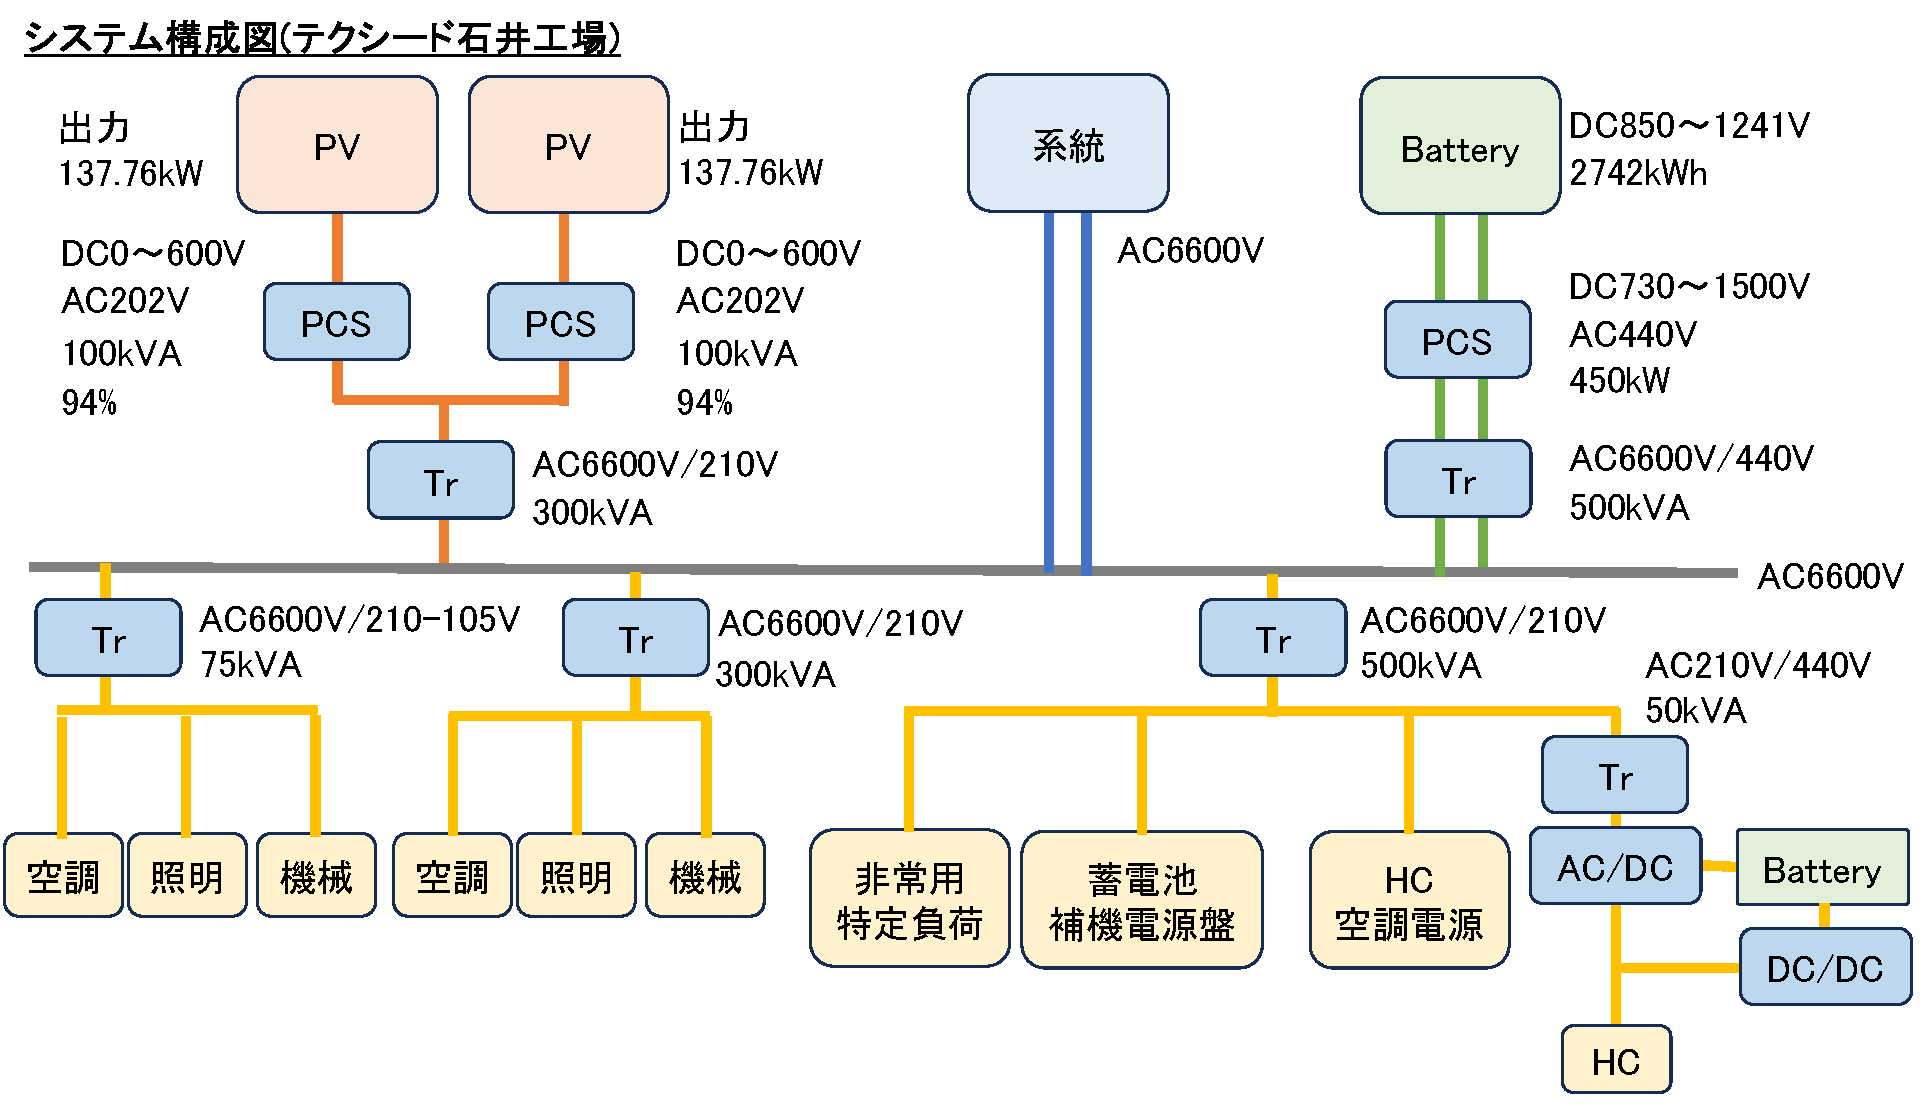
\includegraphics[width=155mm]{../figure/tecseed.pdf}
 \caption{テクシード構成図}
 \label{fig:tecseed}
\end{figure}

\section{線形計画法を用いた場合と動的計画法を用いた場合の計算時間の比較}
「20250703-0721テクシード電力量データ.xlsx」を用いて，線形計画法を用いた場合と動的計画法を用いた場合で
計算時間がどの程度変化するのかを実験した．実験に使用した環境を表\ref{table:environment}に示す．
なお，線形計画モデルについて，決定変数に整数変数やバイナリ変数は含まれておらず，
非線形の制約条件も含まれていない．
計算時間についてはプログラムの開始から最適解を導出するまでの時間である実行時間を計測した．
その内訳として，外部入力に伴う時間と，ソルバーによる最適化を行う時間であるCPU時間に分けた．
各手法各問題の規模で5回計測し，その平均値を採用している．期の数$K$を5040,10080,15120,20160（それぞれの値は1期あたり1分とした場合，0.5週間，1週間，1.5週間，2週間に相当する）と，バッテリーの段階数$B$を6855,13710,27420(それぞれの値はバッテリーの最大容量を2742 kWhとした場合，バッテリーの刻み幅が0.4 kWh，0.2 kWh，0.1kWhである状態に相当する)と変化させながら線形計画法と動的計画法のそれぞれについて計算時間を求めたものを表\ref{table:time_lp}，表\ref{table:time_dp}に示す．

まずは，$K$に注目して考察を行う．表\ref{table:time_lp}より，本問題に対して線形計画法を用いた場合，CPU時間はおおよそ$K$に比例，あるいはそれ以上の次数で増加していることがわかる．ところで，求解アルゴリズムの内ではシンプレックス法が用いられているがシンプレックス法の時間的計算量について，Dantzigらによると「典型的な
反復回数は制約条件の数に比例して増大し(その比例係数は3/2〜3程度)，変数の数に関してはきわめてゆっくりと増大する」といった理論的解釈が提案されている．しかしながら，最悪の場合の反復回数はあくまでも問題の規模に対して指数関数程度的に増加することも知られている．ただし，このようなケースは「病的」ともいわれるほどに特殊なケースであり，現実的な問題のほとんど全てに対してDantzigらによる反復回数の見積もりが有効である．\footnote{玉置久, 『システム最適化』, オーム社, 2005.}
実際，本問題でもおよそ3倍程度の比例定数で$K$に比例してCPU時間が増加している挙動を確認できる．

一方で表\ref{table:time_dp}より，本問題に対して動的計画法を用いた場合，こちらもCPU時間はおおよそ$K$に比例して増加し，その比例係数は1程度になっていることがわかる．実際，本問題に対して動的計画法を用いた場合，時間的計算量は$O(KB^2)$となるため，その通りの結果になっていることが確認できる．以上のことより$K$だけに注目した場合，ある値までは線形計画法の方が高速に問題を解くことが可能であるが，それ以降は動的計画法の方が高速に問題を解くことが可能であると考えられる．

次に$B$に注目して考察を行う．表\ref{table:time_dp}より$B$の数を2倍にするとCPU時間はおおよそ4倍になっていることがわかる．前述したように，
本問題に対して動的計画法を用いた場合，時間的計算量は$O(KB^2)$となるため，その通りの結果になっていることが確認できる．
以上より，$B$の値が小さいときは線形計画法よりも動的計画法のほうが高速に問題を解くことが可能であると考えられるが，
解の精度を高める必要がある場合には，LPの方が有利になる可能性がある．

\begin{table}[htbp]
  \centering
  \caption{実行環境の仕様}
  \label{table:environment}
  \begin{tabular}{ll}
    \hline
    項目 & 内容 \\
    \hline \hline
    CPU & Intel Core i5 1.4 GHz Quad-Core \\
    RAM & 16 GB 2133 MHz\\
    OS & macOS Ventura 13.7.8 \\
    使用言語 & Python 3.9.12\\
    使用ライブラリ(LP,DP共通) & Pandas, NumPy, Matplotlib, os, unicodedata\\ 
     使用ライブラリ(LP) & PySCIPOpt\\
     使用ライブラリ(DP)& Numba\\
    \hline
  \end{tabular}
\end{table}

\begin{table}[htbp]
  \centering
  \caption{計算時間(線形計画法)}
  \label{table:time_lp}
  \begin{tabular}{ccc}
    \hline
    $K$ & 外部入力に伴う時間[s] & CPU時間[s]\\ 
    \hline \hline
     5040 & 2.59 & 7.96\\
    10080 & 4.15& 25.25\\
    15120 &  7.97&44.40\\
    20160 &  10.14&70.60\\
    \hline
  \end{tabular}
\end{table}

\begin{table}[htbp]
  \centering
  \caption{計算時間(動的計画法)}
  \label{table:time_dp}
  \begin{tabular}{cccc}
    \hline
    $K$ &  $B$ & 外部入力に伴う時間[s] & CPU時間[s]\\
    \hline \hline
    5040 & 6855& 2.50 & 5.65\\
    10080 & & 4.29 &10.83 \\
    15120 &  & 6.48 & 14.15\\
    20160 &  & 8.86 & 18.95\\
    5040 & 13710& 2.67 & 18.43\\
    10080 & & 4.42 &34.68 \\
    15120 & & 6.92 & 49.33\\
    20160 & & 9.00 & 67.57\\
     5040 & 27420& 2.60 & 62.64\\
    10080 & & 4.13 &125.03 \\
    15120 & & 6.79 & 180.09\\
    20160 & & 8.90 & 245.12\\
    \hline
  \end{tabular}
\end{table}



\end{document}
